\documentclass[12pt, titlepage]{article}

\usepackage{fullpage}
\usepackage[round]{natbib}
\usepackage{multirow}
\usepackage{booktabs}
\usepackage{tabularx}
\usepackage{graphicx}
\usepackage{float}
\usepackage{pdflscape}
\usepackage{hyperref}
\hypersetup{
    colorlinks,
    citecolor=blue,
    filecolor=black,
    linkcolor=red,
    urlcolor=blue
}

%% Comments

\usepackage{color}

\newif\ifcomments\commentstrue %displays comments
%\newif\ifcomments\commentsfalse %so that comments do not display

\ifcomments
\newcommand{\authornote}[3]{\textcolor{#1}{[#3 ---#2]}}
\newcommand{\todo}[1]{\textcolor{red}{[TODO: #1]}}
\else
\newcommand{\authornote}[3]{}
\newcommand{\todo}[1]{}
\fi

\newcommand{\wss}[1]{\authornote{blue}{SS}{#1}} 
\newcommand{\plt}[1]{\authornote{magenta}{TPLT}{#1}} %For explanation of the template
\newcommand{\an}[1]{\authornote{cyan}{Author}{#1}}

%% Common Parts

\newcommand{\progname}{ProgName} % PUT YOUR PROGRAM NAME HERE
\newcommand{\authname}{Team \#, Team Name
\\ Student 1 name
\\ Student 2 name
\\ Student 3 name
\\ Student 4 name} % AUTHOR NAMES                  

\usepackage{hyperref}
    \hypersetup{colorlinks=true, linkcolor=blue, citecolor=blue, filecolor=blue,
                urlcolor=blue, unicode=false}
    \urlstyle{same}
                                


\newcounter{acnum}
\newcommand{\actheacnum}{AC\theacnum}
\newcommand{\acref}[1]{AC\ref{#1}}

\newcounter{ucnum}
\newcommand{\uctheucnum}{UC\theucnum}
\newcommand{\uref}[1]{UC\ref{#1}}

\newcounter{mnum}
\newcommand{\mthemnum}{M\themnum}
\newcommand{\mref}[1]{M\ref{#1}}
\newcommand{\rt}[1]{\textbf{#1}}

\begin{document}

\title{Module Guide for \progname{}} 
\author{\authname}
\date{\today}

\maketitle

\pagenumbering{roman}

\section{Revision History}

\begin{tabularx}{\textwidth}{p{3cm}p{2cm}X}
\toprule {\bf Date} & {\bf Version} & {\bf Notes}\\
\midrule
Jan 10 & 1.0 & Ayman and Kelly worked on Anticipated changes and introduction\\
Jan 12 & 1.1 & Reza worked on design timeline and the architecture\\
Jan 13 & 1.2 & Nathan completed list of modules and the architecture, and Patrick worked on the module decomposition and the traceability with requirements\\
Jan 16 & 1.3 & General changes given by the feedbacks from TA meetings, and team group meetings to go through\\
Jan 17 & 1.4 & Finalized Document\\
\bottomrule
\end{tabularx}

\newpage

\section{Reference Material}

This section records information for easy reference.

\subsection{Abbreviations and Acronyms}

\renewcommand{\arraystretch}{1.2}
\begin{tabular}{l l} 
  \toprule		
  \textbf{symbol} & \textbf{description}\\
  \midrule 
  AC & Anticipated Change\\
  DAG & Directed Acyclic Graph \\
  M & Module \\
  MG & Module Guide \\
  OS & Operating System \\
  R & Requirement\\
  SC & Scientific Computing \\
  SRS & Software Requirements Specification\\
  \progname & Chest X-Ray scan Analysis\\
  UC & Unlikely Change \\
  \bottomrule
\end{tabular}\\

\newpage

\tableofcontents

\listoftables

\listoffigures

\newpage

\pagenumbering{arabic}

\section{Introduction}

Decomposing a system into modules is a commonly accepted approachh to developing
software.  A module is a work assignment for a programmer or programming
team~\citep{ParnasEtAl1984}.  We advocate a decomposition
based on the principle of information hiding~\citep{Parnas1972a}.  This
principle supports design for change, because the ``secrets'' that each module
hides represent likely future changes.  Design for change is valuable in SC,
where modifications are frequent, especially during initial development as the
solution space is explored.  

Our design follows the rules layed out by \citet{ParnasEtAl1984}, as follows:
\begin{itemize}
\item System details that are likely to change independently should be the
  secrets of separate modules.
\item Each data structure is implemented in only one module.
\item Any other program that requires information stored in a module's data
  structures must obtain it by calling access programs belonging to that module.
\end{itemize}

After completing the first stage of the design, the Software Requirements
Specification (SRS), the Module Guide (MG) is developed~\citep{ParnasEtAl1984}. The MG
specifies the modular structure of the system and is intended to allow both
designers and maintainers to easily identify the parts of the software.
potential readers of this document are as follows:

\begin{itemize}
\item New project members: This document can be a guide for a new project member
  to easily understand the overall structure and quickly find the
  relevant modules they are searching for.
\item Maintainers: The hierarchical structure of the module guide improves the
  maintainers' understanding when they need to make changes to the system. It is
  important for a maintainer to update the relevant sections of the document
  after changes have been made.
\item Designers: Once the module guide has been written, it can be used to
  check for consistency, feasibility, and flexibility. Designers can verify the
  system in various ways, such as consistency among modules, feasibility of the
  decomposition, and flexibility of the design.
\end{itemize}

\noindent The rest of the document is organized as follows. Section
\ref{SecChange} lists the anticipated and unlikely changes of the software
requirements. Section \ref{SecMH} summarizes the module decomposition that
was constructed according to the likely changes. Section \ref{SecConnection}
specifies the connections between the software requirements and the
modules. Section \ref{SecMD} gives a detailed description of the
modules. Section \ref{SecTM} includes two traceability matrices. One checks
the completeness of the design against the requirements provided in the SRS. The
other shows the relation between anticipated changes and the modules. Section
\ref{SecUse} describes the use relation between modules.

% \subsection{Overview}
% This Module Guide Document serves as a design blueprint for CXR - a web-based chest X-ray analysis application developed to support healthcare professionals in diagnosing and monitoring respiratory and cardiac conditions. It provides a modular overview of the project, enabling the development team to build a platform that prioritizes accurate diagnostics, efficient performance, and seamless integration into existing medical workflows.

% \subsection{Purpose}
% The aim of this Module Guide Document is to detail the architecture of modules, based on selected design principles and patterns, to clarify the project’s functionalities and the specific roles of each module.

% \subsection{Design Principles}
% The Module Guide will emphasize modularity, scalability, and separation of concerns for efficient, maintainable design. It promotes reusability, interoperability, and security while ensuring simplicity, robustness, and testability. Consistent standards and traceability will streamline development and maintenance.

\section{Anticipated and Unlikely Changes} \label{SecChange}

This section lists possible changes to the system. According to the likeliness
of the change, the possible changes are classified into two
categories. Anticipated changes are listed in Section \ref{SecAchange}, and
unlikely changes are listed in Section \ref{SecUchange}.

\subsection{Anticipated Changes} \label{SecAchange}

Anticipated changes are adjustments expected during the project lifecycle and are designed to minimize the impact on the overall system. These changes are encapsulated within specific modules to ensure that the modifications affect only the corresponding module. This strategy is referred to as "design for change."

\begin{description}
\item[\refstepcounter{acnum} \actheacnum \label{acHardware}:] The specific hardware configurations on which the AI model runs may evolve as technology advances, including GPU updates for faster computations or better memory handling.

\item[\refstepcounter{acnum} \actheacnum \label{acInput}:] The format or structure of input chest X-rays might vary, such as accommodating different resolutions or adding metadata for enhanced analysis.

\item[\refstepcounter{acnum} \actheacnum \label{acCompliance}:] Changes in healthcare regulations could require modifications to the model’s outputs or data handling to ensure compliance with privacy and security standards.

\item[\refstepcounter{acnum} \actheacnum \label{acDisease}:] Refining the list of detectable diseases as new medical research or datasets become available.

\item[\refstepcounter{acnum} \actheacnum \label{acUI}:] Adjustments to the front-end interface to make it more user-friendly for medical professionals, incorporating feedback from usability studies.

\item[\refstepcounter{acnum} \actheacnum \label{acErrorHandling}:] Introducing or refining mechanisms to manage edge cases, such as incomplete or corrupted input data.

\item[\refstepcounter{acnum} \actheacnum \label{acPreprocessing}:] Enhancements to image preprocessing, such as noise reduction, normalization, or resizing techniques, to improve the quality of input data.

\end{description}

\subsection{Unlikely Changes} \label{SecUchange}

Unlikely changes are those that are not expected to occur during the project lifecycle. These changes typically involve fundamental shifts in the system's scope, technology, or purpose and would require significant effort to implement.


\begin{description}
\item[\refstepcounter{ucnum} \uctheucnum \label{ucFrameworkMigration}:] Switching from PyTorch to an entirely different deep learning framework, such as TensorFlow or JAX, is unlikely due to the associated complexity and cost.

\item[\refstepcounter{ucnum} \uctheucnum \label{ucPurpose}:] A change in the primary use case, such as shifting from diagnostic support to research-oriented predictions, is considered unlikely.

\item[\refstepcounter{ucnum} \uctheucnum \label{ucObjective}:] Shifting the AI model's purpose from disease prediction to a completely different application, such as general image classification.

\item[\refstepcounter{ucnum} \uctheucnum \label{ucNonAI}:] Eliminating the AI model and replacing it with traditional statistical methods or rule-based systems.

\item[\refstepcounter{ucnum} \uctheucnum \label{ucScopeExpansion}:] Expanding the system to predict non-chest-related diseases or conditions beyond its initial design focus or the project's current scope.
\end{description}

\section{Module Hierarchy} \label{SecMH}

This section provides an overview of the module design. Modules are summarized
in a hierarchy decomposed by secrets in Table \ref{TblMH}. The modules listed
below, which are leaves in the hierarchy tree, are the modules that will
actually be implemented.

\begin{description}
\item [\refstepcounter{mnum} \mthemnum \label{mWebApp}:] Web Application 
\item [\refstepcounter{mnum} \mthemnum \label{mHTTP}:] HTTP Server 
\item [\refstepcounter{mnum} \mthemnum \label{mDiseasePredict}:] Disease Prediction Server 
\item [\refstepcounter{mnum} \mthemnum \label{mDiseaseProgress}:] Disease Progression Server
\item [\refstepcounter{mnum} \mthemnum \label{mAuth}:] User Authentication 
\item [\refstepcounter{mnum} \mthemnum \label{mPatientList}:] Patients List View 
\item [\refstepcounter{mnum} \mthemnum \label{mPatientOverview}:] Patient Overview View 
\item [\refstepcounter{mnum} \mthemnum \label{mProgressView}:] Disease Progression View 
\item [\refstepcounter{mnum} \mthemnum \label{mRecordsList}:] Medical Records List View
\item [\refstepcounter{mnum} \mthemnum \label{mReportView}:] X-Ray Report View
\item [\refstepcounter{mnum} \mthemnum \label{mProgressModel}:] Disease Progression Model 
\item [\refstepcounter{mnum} \mthemnum \label{mPredictModel}:] Disease Prediction Model
\item [\refstepcounter{mnum} \mthemnum \label{mRecord}:] Medical Record Management
\item [\refstepcounter{mnum} \mthemnum \label{mDataStore}:] Data Persistent 
\end{description}




\begin{table}[h!]
\centering
\begin{tabular}{p{0.3\textwidth} p{0.6\textwidth}}
\toprule
\textbf{Level 1} & \textbf{Level 2}\\
\midrule

{Hardware-Hiding Module} &  Web Application\\
& HTTP Server \\
& Disease Prediction Server\\
& Disease Progression Server\\
\midrule

\multirow{7}{0.3\textwidth}{Behaviour-Hiding Module} & User Authentication \\
& Patients List View\\
& Patient Overview View \\
& Disease Progression View \\
& Medical Records List View\\
& X-Ray Report View\\
\midrule

\multirow{3}{0.3\textwidth}{Software Decision Module} & Disease Progression Model \\
& Disease Prediction Model\\
& Medical Record Management\\
& Data Persistent \\
\bottomrule

\end{tabular}
\caption{Module Hierarchy}
\label{TblMH}
\end{table}
\newpage
\section{Connection Between Requirements and Design} \label{SecConnection}

The design of the system is intended to satisfy the requirements developed in
the SRS. In this stage, the system is decomposed into modules. The connection
between requirements and modules is explained in detailed below and the traceability is listed in Table~\ref{TblRT}.
 
\subsection{Functional Requirements (FR)}
\textbf{FR1: Accept chest X-ray images as input} \\
Modules: \mref{mDiseasePredict}, \mref{mDiseaseProgress}, \mref{mProgressModel}, \mref{mPredictModel} \\
Rationale: These modules are responsible for processing X-ray images for disease prediction and tracking progression. They handle the image input and its integration into the disease detection pipeline. \\
\newline
\textbf{FR2: Input additional patient symptoms} \\
Modules: \mref{mDiseasePredict}, \mref{mReportView}, \mref{mPredictModel} \\
Rationale: The system requires patient symptoms for disease prediction. \mref{mDiseasePredict} and \mref{mPredictModel} handle the input, while \mref{mReportView} is responsible for displaying the results, including the additional symptoms. \\
\newline
\textbf{FR3: Analyze chest X-rays for disease detection} \\
Modules: \mref{mDiseasePredict}, \mref{mPredictModel} \\
Rationale: These modules perform the core task of analyzing X-rays and predicting disease based on the image content. \\
\newline
\textbf{FR4: Monitor patient condition changes} \\
Modules: \mref{mDiseaseProgress}, \mref{mProgressModel} \\
Rationale: These modules track the progression of a disease over time and analyze changes in the patient’s condition, ensuring that the system provides up-to-date insights into the patient's health. \\
\newline
\textbf{FR5: Highlight affected areas on X-rays} \\
Modules: \mref{mDiseasePredict}, \mref{mReportView}, \mref{mPredictModel} \\
Rationale: \mref{mDiseasePredict} analyzes the X-rays and identifies affected areas, while \mref{mReportView} visualizes those areas for the user. \mref{mPredictModel} assists with disease prediction and highlighting. \\
\newline
\textbf{FR6: Generate a structured report} \\
Modules: \mref{mReportView} \\
Rationale: This module is responsible for generating and displaying structured reports based on the analyzed X-rays and predicted diagnoses. \\
\newline
\textbf{FR7: Store patient data securely} \\
Modules: \mref{mDataStore} \\
Rationale: \mref{mDataStore} is specifically designed to store and manage patient data securely, ensuring compliance with data protection regulations. \\
\newline
\textbf{FR8: Provide alerts for significant condition changes} \\
Modules: \mref{mDiseaseProgress}, \mref{mPatientList}, \mref{mPatientOverview}, \mref{mProgressView} \\
Rationale: These modules monitor changes in a patient's condition and provide notifications when significant changes are detected. They also handle displaying the alerts to users. \\
\newline
\textbf{FR9: Allow treatment plan adjustments} \\
Modules: \mref{mReportView}, \mref{mRecord} \\
Rationale: \mref{mReportView} stores medical records, which includes treatment plans. \mref{mRecord} module enables viewing and adjusting the plans as necessary. \\
\newline
\textbf{FR10: Integrate with EHR systems} \\
Modules: \mref{mRecord}, \mref{mDataStore} \\
Rationale: Integration with EHR (Electronic Health Records) systems requires a secure and reliable data storage mechanism, handled by the \mref{mRecord} and \mref{mDataStore} module. \\
\newline
\textbf{FR11: Display confidence levels in UI} \\
Modules: \mref{mReportView} \\
Rationale: The confidence levels of AI predictions are displayed through the \mref{mReportView} to inform users about the accuracy of diagnoses. \\
\newline
\textbf{FR12: Patient uploads for self-diagnosis (Canceled)} \\
Rationale: This feature was canceled, so no module is connected to it. \\
\newline
\textbf{FR13: Support user roles and access levels (Canceled)} \\
Rationale: This feature was canceled, so no module is connected to it. \\
\newline
\textbf{FR14: Create a new copy of X-rays for analysis} \\
Modules: \mref{mRecordsList} \\
Rationale: The \mref{mRecordsList} module manages and stores medical records, including X-ray images, and enables creating new copies for further analysis. \\
\newline
\textbf{FR15: Support AI model updates} \\
Modules: \mref{mDiseasePredict}, \mref{mDiseaseProgress}, \mref{mProgressModel}, \mref{mPredictModel} \\
Rationale: These modules rely on AI models for disease prediction and progression analysis. The system needs to support updates to these models as new data or improvements emerge. \\
\newline
\subsection{Non-Functional Requirements (NFR)}
\textbf{LF1: Consistent user interface} \\
Modules: \mref{mPatientList}, \mref{mPatientOverview}, \mref{mProgressView}, \mref{mRecordsList} \\
Rationale: These modules are essential for maintaining a consistent UI across the system, ensuring a seamless user experience for viewing patient details and progress. \\
\newline
\textbf{LF2: Ergonomic color schemes and fonts} \\
Modules: \mref{mPatientList}, \mref{mPatientOverview}, \mref{mProgressView}, \mref{mRecordsList} \\
Rationale: These modules focus on presenting patient data and disease progression in an easy-to-read, ergonomic manner. Consistent color schemes and font choices are critical for a good user experience. \\
\newline
\textbf{UH1: Usability for common tasks} \\
Modules:\mref{mPatientList}, \mref{mPatientOverview}, \mref{mProgressView}, \mref{mRecordsList}\\
Rationale: These modules are designed with usability in mind to allow healthcare professionals to perform tasks such as searching for patients, viewing records, and analyzing disease progression efficiently. \\
\newline
\textbf{UH2: Context-sensitive help} \\
Modules: \mref{mAuth}, \mref{mDataStore} \\
Rationale: The \mref{mAuth} module ensures that users can access the system securely, while \mref{mDataStore} can provide relevant help regarding data management and privacy settings. \\
\newline
\textbf{PR1: Process images within 30 seconds} \\
Modules: \mref{mDiseasePredict}, \mref{mDiseaseProgress}, \mref{mProgressModel}, \mref{mPredictModel} \\
Rationale: These modules must process images quickly to meet the 30-second time constraint for efficient diagnosis and progression tracking. \\
\newline
\textbf{PR2: Maintain consistent availability} \\
Modules: \mref{mWebApp}, \mref{mHTTP} \\
Rationale: These modules ensure that the application is available and responsive at all times, minimizing downtime for users who rely on the system. \\
\newline
\textbf{PR3: Concurrent processing of 20 images} \\
Modules: \mref{mDiseasePredict}, \mref{mDiseaseProgress}, \mref{mProgressModel}, \mref{mPredictModel} \\
Rationale: The system is designed to handle the simultaneous processing of multiple images, enabling efficient analysis of large batches of X-rays or other diagnostic images. \\
\newline
\textbf{OE1: Integration with PACS systems} \\
Modules: \mref{mDataStore} \\
Rationale: PACS (Picture Archiving and Communication System) integration allows the system to interact with medical imaging databases, which is managed by \mref{mDataStore}. \\
\newline
\textbf{OE2: Operate in variable network conditions} \\
Modules: \mref{mWebApp}, \mref{mHTTP} \\
Rationale: These modules are built to handle different network conditions, ensuring that the web application can function reliably even with fluctuating internet speeds. \\
\newline
\textbf{SR1: Encrypt patient data} \\
Modules: \mref{mDataStore} \\
Rationale: \mref{mDataStore} ensures that patient data is encrypted both in transit and at rest, satisfying security and privacy regulations. \\
\newline
\textbf{MS1: Modular architecture} \\
Modules: \mref{mReportView}, \mref{mProgressModel}, \mref{mPredictModel} \\
Rationale: The modular architecture allows each module to be updated or replaced independently, facilitating maintenance and scalability. \\
\newline
\textbf{MS2: Automated testing suites} \\
Modules: \mref{mDiseasePredict}, \mref{mDiseaseProgress}, \mref{mProgressModel}, \mref{mPredictModel}, \mref{mRecord} \\
Rationale: These modules require robust automated testing to ensure their functionality and accuracy in disease prediction, progression tracking, and data management. \\
\newline
\textbf{CR1: Support English and French languages} \\
Modules: \mref{mPatientList}, \mref{mPatientOverview}, \mref{mProgressView}, \mref{mRecordsList}, \mref{mReportView} \\
Rationale: These modules display patient information and reports, which must support multiple languages for broader user accessibility. \\
\newline
\textbf{LR1: Compliance with healthcare data protection laws} \\
Modules: \mref{mDataStore} \\
Rationale: \mref{mDataStore} ensures compliance with healthcare regulations by securely handling patient data in accordance with legal requirements. \\
\newline
\textbf{LR2: Adherence to ISO 13485} \\
Modules: \mref{mDataStore} \\
Rationale: \mref{mDataStore} ensures that all data handling and storage comply with ISO 13485 standards for medical devices. \\
\newline
\textbf{HS1: Radiologist validation of AI-generated diagnoses} \\
Modules: \mref{mReportView} \\
Rationale: The \mref{mReportView} module provides a platform for radiologists to review AI-generated diagnoses and confirm their accuracy before taking action. \\
\newline
\textbf{HS2: Clear disclaimers about AI limitations} \\
Modules: \mref{mReportView} \\
Rationale: \mref{mReportView} includes disclaimers in the generated reports to inform users about the limitations of AI-based predictions. \\

\section{Module Decomposition} \label{SecMD}

Modules are decomposed according to the principle of ``information hiding''
proposed by \citet{ParnasEtAl1984}. The \emph{Secrets} field in a module
decomposition is a brief statement of the design decision hidden by the
module. The \emph{Services} field specifies \emph{what} the module will do
without documenting \emph{how} to do it. For each module, a suggestion for the
implementing software is given under the \emph{Implemented By} title. If the
entry is \emph{OS}, this means that the module is provided by the operating
system or by standard programming language libraries.  \emph{\progname{}} means the
module will be implemented by the \progname{} software.
\newline
Only the leaf modules in the hierarchy have to be implemented. If a dash
(\emph{--}) is shown, this means that the module is not a leaf and will not have
to be implemented.

\subsection{Hardware-Hiding Modules}
\begin{description}
\item[Secrets:] The data structures and algorithms used to implement the virtual hardware layer that abstracts infrastructure complexities.
\item[Services:] Provides virtualized hardware interfaces to the rest of the system, enabling hardware-independent operation.
\item[Implemented By:] --
\end{description}

\subsubsection{Web Application Server Module (\mref{mWebApp})}
\begin{description}
\item[Secrets:] The web server implementation and configuration details for handling web UI requests.
\item[Services:] Provides a platform for hosting and serving the web application to users.
\item[Implemented By:] Docker Engine
\end{description}

\subsubsection{HTTP Server Module (\mref{mHTTP})}
\begin{description}
\item[Secrets:] The implementation details of HTTP protocol handling and network communication.
\item[Services:] Provides HTTP communication interface for client-server interactions.
\item[Implemented By:] Docker Engine
\end{description}

\subsubsection{Disease Prediction Server Module (\mref{mDiseasePredict})}
\begin{description}
\item[Secrets:] The implementation details of GPU resource management and ML model pipeline.
\item[Services:] Provides computational resources for disease prediction model execution.
\item[Implemented By:] Docker Engine and CUDA
\end{description}

\subsubsection{Disease Progression Server Module (\mref{mDiseaseProgress})}
\begin{description}
\item[Secrets:] The implementation details of parallel processing and GPU resource allocation for temporal progression analysis.
\item[Services:] Provides computational resources for disease progression analysis.
\item[Implemented By:] Docker Engine and CUDA
\item[Type of Module:] Hardware-Hiding
\end{description}

\subsection{Behaviour-Hiding Module}

\begin{description}
\item[Secrets:]The contents of the required behaviours.
\item[Services:]Includes programs that provide externally visible behaviour of
  the system as specified in the software requirements specification (SRS)
  documents. This module serves as a communication layer between the
  hardware-hiding module and the software decision module. The programs in this
  module will need to change if there are changes in the SRS.
\item[Implemented By:] --
\end{description}

\subsubsection{User Authentication Module (\mref{mAuth})}
\begin{description}
\item[Secrets:] AWS Cognito integration patterns and frontend authentication workflows that handle secure medical staff access.
\item[Services:] Provides a secure gateway for medical personnel to access the system through login forms, handles session persistence, and manages role-based access control.
\item[Implemented By:] React, JavaScript, and AWS Cognito
\item[Type of Module:] Abstract Object
\end{description}

\subsubsection{Patient List View Module (\mref{mPatientList})}
\begin{description}
\item[Secrets:] Component architecture for displaying and managing tabular patient data with sorting and filtering capabilities.
\item[Services:] Renders an interactive table interface displaying patient records with customizable columns. Enables medical staff to quickly sort, filter, and search through patient lists while maintaining responsive performance.
\item[Implemented By:] React and JavaScript
\item[Type of Module:] Abstract Object
\end{description}

\subsubsection{Patient Overview View Module (\mref{mPatientOverview})}
\begin{description}
\item[Secrets:] Dynamic data presentation based on patient's overall medical condition and historical data.
\item[Services:] Displays a summary of the patient's information, including diagnoses, medications, and treatment progress .
\item[Implemented By:] React and JavaScript
\item[Type of Module:] Abstract Object
\end{description}

\subsubsection{Disease Progression View Module (\mref{mProgressView})}
\begin{description}
\item[Secrets:] Side by side comparison of 2 X-Ray records.
\item[Services:] Displays the disease progression of the patient over 2 selected X-Ray records.
\item[Implemented By:] React and JavaScript
\item[Type of Module:] Abstract Object
\end{description}

\subsubsection{Patient Medical Records List View Module (\mref{mRecordsList})}
\begin{description}
\item[Secrets:] Virtual scrolling implementation and lazy loading patterns for efficient record display.
\item[Services:] Manages the presentation of paginated medical records detailing the patient's medical history.
\item[Implemented By:] React and JavaScript
\item[Type of Module:] Abstract Object
\end{description}

\subsubsection{X-Ray Report View Module (\mref{mReportView})}
\begin{description}
\item[Secrets:] Form layout and validation logic for structured medical report display.
\item[Services:] Presents AI generated reports in a structured format with detailing the findings of the X-Ray.
\item[Implemented By:] React and JavaScript
\item[Type of Module:] Abstract Object
\end{description}


\subsection{Software Decision Module}

\begin{description}
\item[Secrets:] The design decision based on mathematical theorems, physical
  facts, or programming considerations. The secrets of this module are
  \emph{not} described in the SRS.
\item[Services:] Includes data structure and algorithms used in the system that
  do not provide direct interaction with the user. 
\item[Implemented By:] --
\end{description}

\subsubsection{Disease Progression Model Module (\mref{mProgressModel})}
\begin{description}
\item[Secrets:] The criteria and methods for detecting and quantifying changes in disease manifestation between X-ray images over time.
\item[Services:] Analyzes temporal changes in specific lung regions using DETR(Detection Transformer) for precise disease progression monitoring.
\item[Implemented By:] PyTorch
\item[Type of Module:] Abstract Object
\end{description}

\subsubsection{Disease Prediction Model Module (\mref{mPredictModel})}
\begin{description}
\item[Secrets:] The algorithm used to identify diseases and their severity from X-ray image features.
\item[Services:] Processes chest X-ray images to provide disease classification and severity scores using a fine-tuned ResNet model.
\item[Implemented By:] PyTorch
\item[Type of Module:] Abstract Object
\end{description}

\subsubsection{Medical Record Management Module (\mref{mRecord})}
\begin{description}
\item[Secrets:] Record data structure organization, state management patterns, and client-side caching strategies for efficient record handling and display.
\item[Services:] Manages medical record data operations including creation, updates, and retrieval of patient records, prescriptions, and associated medical history while maintaining data consistency.
\item[Implemented By:] Flask
\item[Type of Module:] Abstract Object
\end{description}

\subsubsection{Data Persistence Module (\mref{mDataStore})}
\begin{description}
\item[Secrets:] The organization and relationships between different types of patient data, and the rules for maintaining data consistency and accessibility.
\item[Services:] Manages data storage and retrieval using AWS S3 for Patient Data including X-Ray Images, prescriptions, clinical notes, and DynamoDB for structured data.
\item[Implemented By:] AWS S3 and DynamoD
\item[Type of Module:] Abstract Object
\end{description}


\section{Traceability Matrix} \label{SecTM}

This section shows two traceability matrices: between the modules and the
requirements and between the modules and the anticipated changes.

% the table should use mref, the requirements should be named, use something
% like fref
\begin{table}[H]
\centering
\begin{tabular}{p{0.6\textwidth} p{0.3\textwidth}}
\toprule
\textbf{Req.} & \textbf{Modules}\\
\midrule
FR1: Accept chest X-ray images as input & \mref{mDiseasePredict}, \mref{mDiseaseProgress}, \mref{mProgressModel}, \mref{mPredictModel}\\
FR2: Input additional patient symptoms & \mref{mDiseasePredict}, \mref{mPredictModel}\\
FR3: Analyze chest X-rays for disease detection & \mref{mDiseasePredict}, \mref{mPredictModel}\\
FR4: Monitor patient condition changes & \mref{mDiseaseProgress}, \mref{mProgressModel}\\
FR5: Highlight affected areas on X-rays & \mref{mDiseasePredict}, \mref{mReportView}, \mref{mPredictModel}\\
FR6: Generate a structured report & \mref{mReportView}\\
FR7: Store patient data securely & \mref{mDataStore}\\
FR8: Provide alerts for significant condition changes & \mref{mDiseaseProgress}, \mref{mPatientList}, \mref{mPatientOverview}, \mref{mProgressView}\\
FR9: Allow treatment plan adjustments & \mref{mReportView}, \mref{mRecord}\\
FR10: Integrate with EHR systems & \mref{mRecord}, \mref{mDataStore}\\
FR11: Display confidence levels in UI & \mref{mReportView}\\
FR12: Patient uploads for self-diagnosis (Canceled) & \\
FR13: Support user roles and access levels (Canceled) & \\
FR14: Create a new copy of X-rays for analysis & \mref{mRecordsList}\\
FR15: Support AI model updates & \mref{mDiseasePredict}, \mref{mDiseaseProgress}, \mref{mProgressModel}, \mref{mPredictModel}\\
\bottomrule
\end{tabular}
\caption{Trace Between Functional Requirements and Modules}
\label{TblRT}
\end{table}


\begin{table}[H]
\centering
\begin{tabular}{p{0.6\textwidth} p{0.3\textwidth}}
\toprule
\textbf{Requirement} & \textbf{Modules} \\
\midrule
LF1: Consistent user interface &\mref{mPatientList}, \mref{mPatientOverview}, \mref{mProgressView}, \mref{mRecordsList} \\
LF2: Ergonomic color schemes and fonts & \mref{mPatientList}, \mref{mPatientOverview}, \mref{mProgressView}, \mref{mRecordsList}\\
UH1: Usability for common tasks & \mref{mPatientList}, \mref{mPatientOverview}, \mref{mProgressView}, \mref{mRecordsList}\\
UH2: Context-sensitive help & \mref{mAuth}, \mref{mDataStore} \\
PR1: Process images within 30 seconds & \mref{mDiseasePredict}, \mref{mDiseaseProgress}, \mref{mProgressModel}, \mref{mPredictModel} \\
PR2: Maintain consistent availability & \mref{mWebApp}, \mref{mHTTP} \\
PR3: Concurrent processing of 20 images & \mref{mDiseasePredict}, \mref{mDiseaseProgress}, \mref{mProgressModel}, \mref{mPredictModel} \\
OE1: Integration with PACS systems & \mref{mDataStore} \\
OE2: Operate in variable network conditions & \mref{mWebApp}, \mref{mHTTP} \\
SR1: Encrypt patient data & \mref{mDataStore} \\
SR2: Role-based access control (Canceled) & \\
MS1: Modular architecture & \mref{mReportView}, \mref{mProgressModel}, \mref{mPredictModel} \\
MS2: Automated testing suites & \mref{mDiseasePredict}, \mref{mDiseaseProgress}, \mref{mProgressModel}, \mref{mPredictModel}, \mref{mRecord} \\
CR1: Support English and French languages & \mref{mPatientList}, \mref{mPatientOverview}, \mref{mProgressView}, \mref{mRecordsList}, \mref{mReportView}\\
LR1: Compliance with healthcare data protection laws & \mref{mDataStore} \\
LR2: Adherence to ISO 13485 & \mref{mDataStore} \\
HS1: Radiologist validation of AI-generated diagnoses & \mref{mReportView} \\
HS2: Clear disclaimers about AI limitations & \mref{mReportView} \\
\bottomrule
\end{tabular}
\caption{Trace Between Non-Functional Requirements and Modules}
\label{TblNFRModules}
\end{table}



\begin{table}[H]
\centering
\begin{tabular}{p{0.2\textwidth} p{0.6\textwidth}}
\toprule
\textbf{AC} & \textbf{Modules}\\
\midrule
\acref{acHardware} & \mref{mDiseasePredict}, \mref{mDiseaseProgress}, \mref{mProgressModel}, \mref{mPredictModel}\\
\acref{acInput} & \mref{mDiseasePredict}, \mref{mDiseaseProgress}, \mref{mPatientOverview}, \mref{mProgressView}, \mref{mProgressModel}, \mref{mPredictModel}, \mref{mRecord}\\
\acref{acCompliance} & \mref{mDataStore}\\
\acref{acDisease} & \mref{mDiseasePredict}, \mref{mDiseaseProgress}, \mref{mPredictModel}, \mref{mProgressModel}\\
\acref{acUI} & \mref{mPatientList}, \mref{mPatientOverview}, \mref{mProgressView}, \mref{mRecordsList},\mref{mReportView}\\
\acref{acErrorHandling} & \mref{mDiseasePredict}, \mref{mDiseaseProgress}, \mref{mProgressModel}, \mref{mPredictModel}\\
\acref{acPreprocessing} & \mref{mDiseasePredict}, \mref{mDiseaseProgress}, \mref{mProgressModel}, \mref{mPredictModel}\\
\bottomrule
\end{tabular}
\caption{Trace Between Anticipated Changes and Modules}
\label{TblACT}
\end{table}

\begin{landscape}
\section{Use Hierarchy Between Modules} \label{SecUse}
In this section, the uses hierarchy between modules is
provided. \citet{Parnas1978} said of two programs A and B that A {\em uses} B if
correct execution of B may be necessary for A to complete the task described in
its specification. That is, A {\em uses} B if there exist situations in which
the correct functioning of A depends upon the availability of a correct
implementation of B.  Figure \ref{FigUH} illustrates the use relation between
the modules. It can be seen that the graph is a directed acyclic graph
(DAG). Each level of the hierarchy offers a testable and usable subset of the
system, and modules in the higher level of the hierarchy are essentially simpler
because they use modules from the lower levels. For viewing the image with more clarity please \href{https://github.com/RezaJodeiri/CXR-Capstone/blob/nathan/doc/design/docs/assets/ContextDesignFlow.png}{click here}.
\begin{figure}[H]
\centering
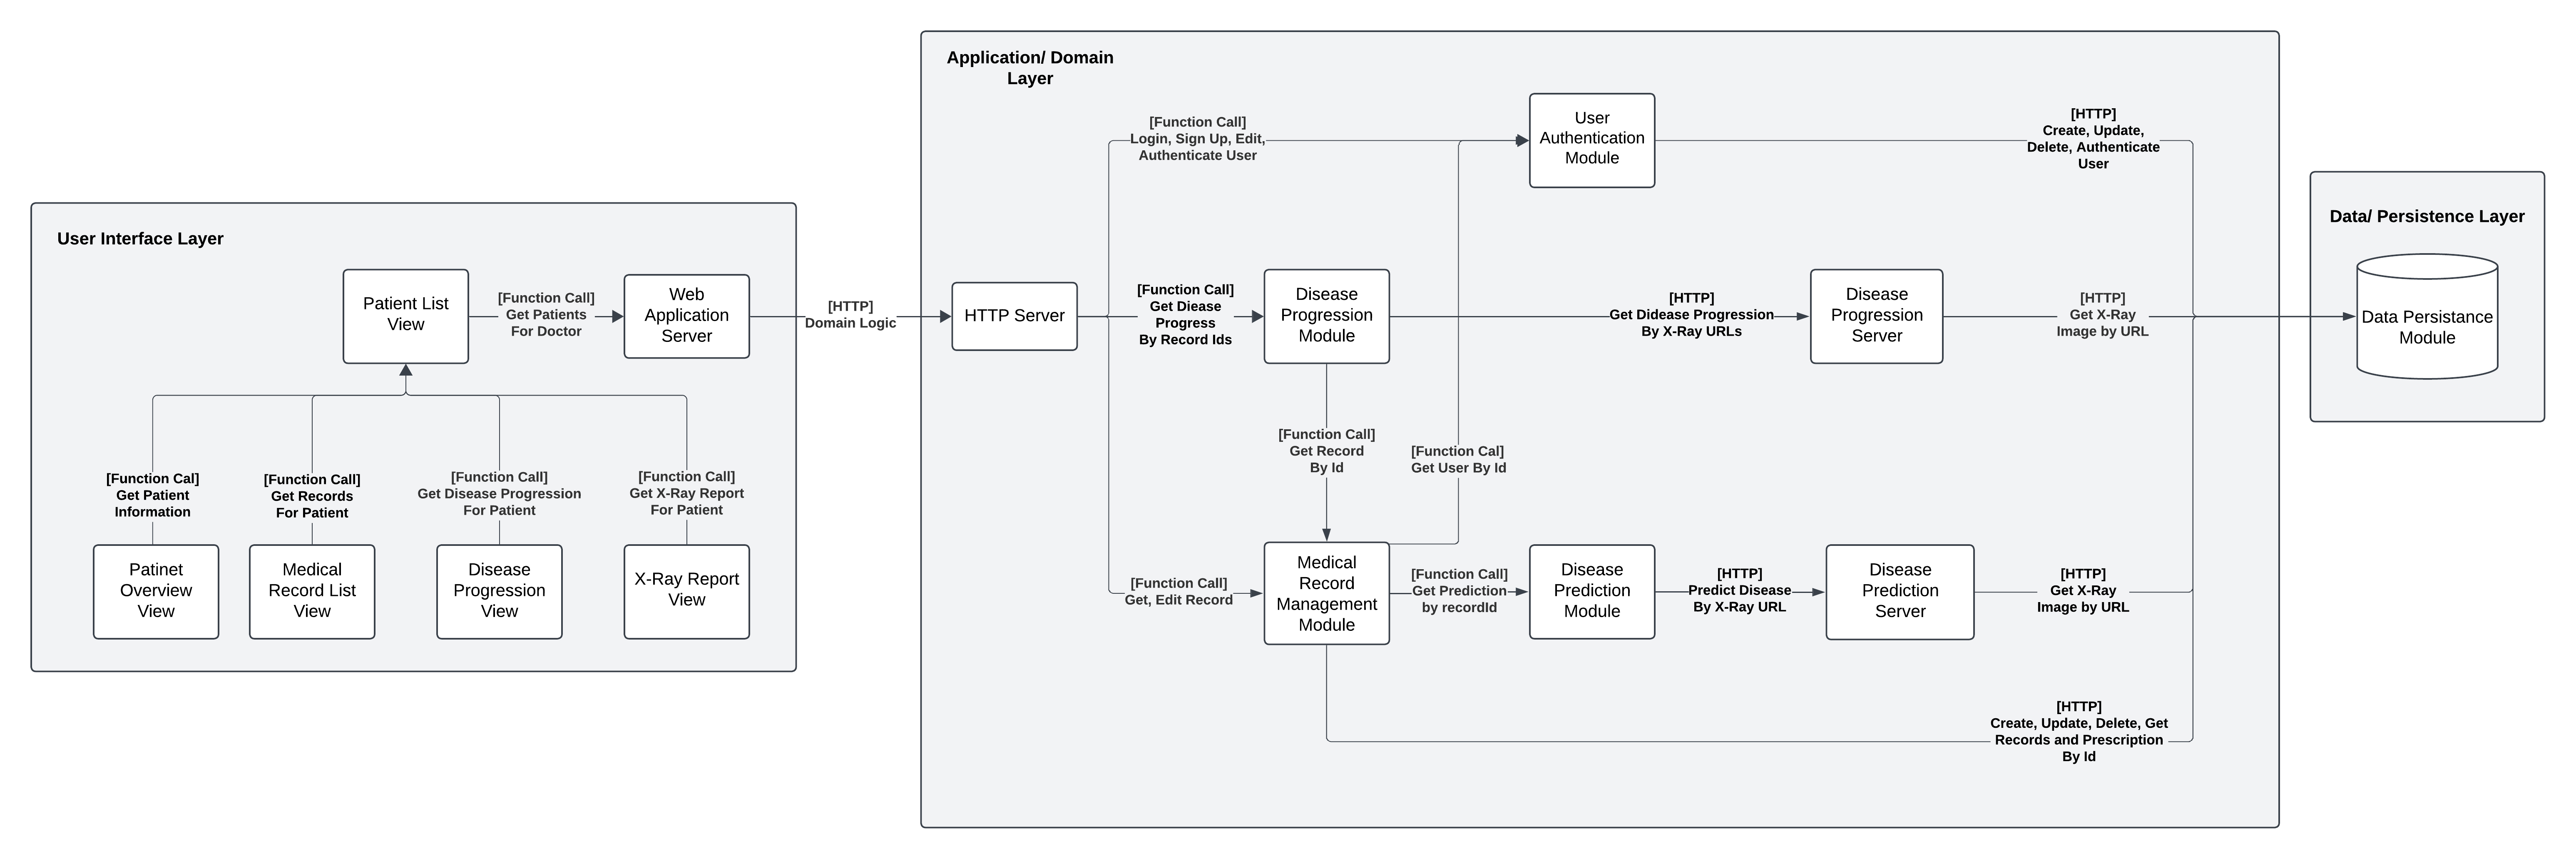
\includegraphics[width=1.45\textwidth]{../../assets/ContextDesignFlow.png}
\caption{Use Hierarchy Diagram showing module interactions}
\label{FigUH}
\end{figure}
\end{landscape}
\subsection{Architecture Summary}
\noindent This system is organized into three main layers---a User Interface layer, an Application/Domain layer, and a Data Persistence layer---each with clear responsibilities and well-defined interfaces:

\begin{enumerate}
    \item \textbf{User Interface Layer} \\
    This layer provides all patient-facing and clinician-facing views. For example, the Patient List View, Patient Overview View, Medical Record List View, Disease Progression View, and X-Ray Report View each issue function calls (e.g., ``Get Patient Information,'' ``Get Records for Patient,'' etc.) to request data and operations.These views communicate with the Web Application Server in the Application/Domain layer.

    \item \textbf{Application/Domain Layer} \\
    At this layer, the Web Application Server routes requests to the HTTP Server, which in turn orchestrates calls to the core modules:
    \begin{itemize}
        \item[-] \textbf{User Authentication Module} -- Manages user login, sign-up, edit, and authentication.
        \item[-] \textbf{Disease Progression Module} -- Retrieves and processes progression data, possibly delegating to the external Disease Progression Server via HTTP.
        \item[-] \textbf{Disease Prediction Module} -- Handles machine-learning predictions for patient records, again leveraging an external Disease Prediction Server.
        \item[-] \textbf{Medical Record Management Module} -- Allows creating, reading, editing, and deleting patient records and prescriptions.
    \end{itemize}
    These modules may also request X-ray images from the Data Persistence layer or send them to the Disease Progression / Prediction servers for further analysis.

    \item \textbf{Data Persistence Layer} \\
    The Data Persistence Module handles storage and retrieval of patient information, records, and X-ray images. All modules in the Application/Domain layer can communicate with this layer to read or persist data as needed.
\end{enumerate}

\noindent By separating concerns into these three layers, the architecture remains modular, enabling independent development, testing, and maintenance of each layer while also decoupling the disease prediction and progression machine learning models.
% \begin{figure}[H]
% \centering
% %\includegraphics[width=0.7\textwidth]{UsesHierarchy.png}
% % \caption{Use hierarchy among modules}
% % \label{FigUH}
% % \end{figure}

%\section*{References}

\newpage
\section{User Interfaces}
The user interface design consists of several key pages that have been prototyped in Figma:

\begin{itemize}
\item A login page for secure user authentication
\item A dashboard showing critical patient statistics and recent X-rays
\item A patient records page displaying medical history and X-ray images
\item A detailed X-ray analysis page with disease detection results
\item A report generation page for doctors to document findings and prescriptions
\item A disease progression tracking interface to monitor changes over time
\end{itemize}

The complete interactive mockups can be viewed at \href{https://www.figma.com/design/HAjX8dhwPjPSzX2Wz06YQ2/Capstone-App?node-id=134-122&t=8ET1qlba7wlarEvq-0}{our Figma design}.

\section{Timeline}
NOTE: M\# in this case stands for milestones.
\begin{itemize} \item \textbf{Week 1 - 2:} \rt{Jan 15 - Jan 28, 2025} \begin{itemize} \item \textbf{M1: Backend Integration Module} \begin{itemize} \item Setup initial backend services for user data, medical records, and X-ray storage (\textit{Nathan}) \item Integrate existing frontend structure with backend endpoints (ensure authentication, data fetching) (\textit{Nathan}) \item Basic testing to confirm data flow and API correctness (\textit{Nathan, Ayman}) \end{itemize} \item \textbf{M2: Report Page Module} \begin{itemize} \item Design the UI/UX for the doctor’s report page (wireframes, user flow) (\textit{Ayman}) \item Implement editable fields (findings, prescriptions, clinical notes) and “Generate Report” functionality (\textit{Ayman}) \item Basic integration tests to ensure the generated report is saved/retrieved properly from backend (\textit{Ayman}) \end{itemize} \end{itemize}

\item \textbf{Week 3 - 4:} \rt{Jan 29 - Feb 11, 2025} \begin{itemize} \item \textbf{M3: Disease Model Implementation Module} \begin{itemize} \item Fine-tune a baseline ML model (e.g., EfficientNet or similar) for disease detection (\textit{Patrick}) \item Incorporate clinical notes or prescription data as additional input (if feasible) (\textit{Patrick}) \item Initial inference endpoint set up in the backend (possibly behind an API route) (\textit{Nathan}) \item Minimal validation tests: confirm the model loads, infers, and returns results (\textit{All as needed}) \end{itemize} \item \textbf{M4: Disease Progression Feature Module} \begin{itemize} \item Research and define approach for tracking disease progression over time (\textit{Reza}) \item Implement backend logic to compare multiple patient X-rays or relevant data points (\textit{Reza}) \item Update UI to support selecting multiple images or timepoints (\textit{Reza}) \item Basic tests for progression calculations (mock data sets, verifying progression output) (\textit{Reza, Nathan}) \end{itemize} \end{itemize}

\item \textbf{Week 5 - 6:} \rt{Feb 12 - Feb 25, 2025} \begin{itemize} \item \textbf{M5: ML related Module} \begin{itemize} \item Collaborate with \textit{Patrick} to gather model outputs for test sets (\textit{Kelly}) \item Develop scripts or a mini-dashboard to compute ROC/AUC, precision/recall, etc. (\textit{Kelly, Patrick}) \item Display these metrics in a UI page or console logs for internal evaluation (\textit{Kelly, Ayman}) \item Run spot checks on real or synthetic data to validate model performance (\textit{Kelly, Patrick}) \end{itemize} \item \textbf{M6: Records list Module} \begin{itemize} \item Design a dashboard that displays quick stats: critical cases, aggregated disease predictions, etc. (\textit{Kelly, Ayman}) \item Implement data retrieval from backend to highlight urgent patient statuses (\textit{Kelly, Nathan}) \item Optional advanced features (if time allows): interactive charts, patient filtering (\textit{Kelly, Ayman}) \end{itemize} \end{itemize}

\item \textbf{Week 7 - 8:} \rt{Feb 26 - Mar 10, 2025} \begin{itemize} \item \textbf{M7: CI/CD Pipeline and Testing Related Modules} \begin{itemize} \item Set up automated build and deployment scripts (GitHub Actions, Jenkins, or similar) (\textit{Ayman}) \item Establish unit and integration test frameworks in both frontend and backend (\textit{Ayman, All team members}) \item Generate code coverage reports and ensure critical paths are tested (\textit{Ayman}) \item Basic load or stress tests on the main endpoints to ensure reliability (\textit{All team members as needed}) \end{itemize} \item \textbf{M8: Finishing Incomplete UI Pages} \begin{itemize} \item Complete Settings/Help page: user preferences, contact info, help content (\textit{Ayman, All team members}) \item Finalize Profile pages: doctor or patient profile editing, access controls (\textit{Ayman, All team members}) \item Ensure consistent styling/theme across all UI pages (\textit{All team members}) \end{itemize} \end{itemize}

\item \textbf{Week 9 - 10:} \rt{Mar 11 - Mar 24, 2025} \begin{itemize} \item \textbf{M9: Additional Sidebar Features} \begin{itemize} \item Add quick links (e.g., “New Report,” “View Dashboard,” “Disease Progression”) strictly relevant to the X-ray project (\textit{Ayman, All team members}) \item Remove or hide unrelated placeholders (appointments, scheduling) to keep UI focused (\textit{Ayman}) \item Small UX improvements (icon updates, rearranging submenus, etc.) (\textit{Ayman}) \end{itemize} \item \textbf{M10: Consolidation and Light Testing} \begin{itemize} \item Review each module’s functionality to ensure “Rev 0” completeness (\textit{All team members}) \item Perform partial integration testing across backend-frontend flows (uploading X-rays, generating reports, disease progression) (\textit{All team members}) \item Document known issues and quick fixes for final refinements (\textit{All team members}) \end{itemize} \end{itemize}

\item \textbf{Week 11 - 12:} \rt{Mar 25 - Apr 7, 2025} \begin{itemize} \item \textbf{M11: Final Checks and Rev 0 Confidence} \begin{itemize} \item Compile partial test results to ensure stable performance (\textit{Ayman, All team members}) \item Confirm ML model accuracy is acceptable; refine or retrain if major gaps found (\textit{ Kelly}) \item Ensure final UI/UX for the doctor’s workflow is coherent (report generation, patient overview, dashboard) (\textit{Ayman}) \item If time allows, address any low-priority enhancements or bugs (\textit{All team members}) \end{itemize} \end{itemize} \end{itemize}

\noindent \textbf{Notes and Assignments Summary:} \begin{itemize} \item \textit{Nathan (Backend Integration)}: AWS S3 setup, database connections, API routes, ensuring the frontend can properly fetch and save data.
\item \textit{Ayman (Frontend UI/UX)}: Report page design/coding, dashboard, overall UI refinement.
\item \textit{Patrick (Disease Model)}: ML model development, fine-tuning, integration into backend inference endpoints.
\item \textit{Reza (Disease Progression)}: Algorithm/design for progression logic, backend integration.
\item \textit{Kelly (ML Metrics, Dashboard Features)}: ROC/AUC, precision/recall metrics, supporting the model team, building quick metrics display.
\item \textit{Ayman (CI/CD, Testing)}: Automate builds, set up test frameworks, code coverage, minimal performance checks.
\item \textit{All Team Members}: Contribute to tests for each feature, help refine UI and fix bugs as needed. \end{itemize}

\noindent By the end of \textbf{Week 12}, we aim for a functional “Rev 0” where doctors can: \begin{itemize} \item Log in to the system
\item Upload or view X-ray images
\item Receive disease predictions and progression analysis
\item Generate and edit a final report (with prescriptions/notes), automatically linked in the patient’s record
\item See basic metrics (ROC/AUC) for the ML model’s performance
\item Use a partially tested, but stable, CI/CD pipeline that automates builds/deployments
\end{itemize}

\noindent Additional refinement or advanced features can be scheduled for post-Rev-0 milestones if time permits.
formation is included there

\bibliographystyle {plainnat}
\bibliography{../../../refs/References}

\newpage{}

\end{document}